\documentclass{myBeamer}

%% Title page
\title{Challenge Scenario}
\subtitle{Zombie Antidote}
\author{}
\date{June 26, 2019}
%\institute{Institut\\
%\bigskip
%
\includegraphics[scale=2]{figures/logos/openmole.png}}

\newcommand{\FL}[1]{\textcolor{red}{#1}}


\begin{document}

\begin{frame}[plain]
	\titlepage
\end{frame}
\addtocounter{framenumber}{-1}

\AtBeginSection[]
{
	\frame{
		\sectionpage
	}
	\addtocounter{framenumber}{-1}
}


\section{Story}

\sframe{Red Cross}{

There are some agents carrying a zombie \textbf{antidote}. When they are alerted to the zombie attack, they take the antidote.

\bigskip
This antidote has an \textbf{activation delay}. Before the actual activation, agents are weaker than normal humans. After activation, they are back to their normal stamina and they are immunized to zombie infection.
}



\sframe{Specificities of antidoters}{

Alert mechanism:
\begin{itemize}
\item They become alerted individually when they  see a zombie.
\end{itemize}
%- all become alerted when one of them sees a zombie (via walkie-talkie) : we do not study this mecanism in the following, tracks for the challenge ? 

\bigskip

When they are immunized, they have specific behaviors:
\begin{itemize}
\item They alert everyone they meet.
\item They run towards zombies to lure them away from normal humans: once a zombie detect an antidoter, he attacks him and they remain face to face for the future steps.
\end{itemize}

}


%\begin{itemize}
%\item 
%\item 
%\end{itemize}


\sframe{New parameters, we can act on}{

\begin{itemize}
\item Number of antidoters: $redCrossSize$ 
\item  Delay of activation of the antidote: $redCrossActivationDelay$
\item  Efficiency of the antidote: $redCrossEfficiencyProbability$
\item  Exhaustion probability modified during activation: $redCrossExhaustionProbability$. Being immunized decreases the stamina of antidoter during the period of activation.
\end{itemize}

By default, we consider the parameter $redCrossInformProbability$ set equal to 1: antidoters transmit their information to every human they meet.

}



%\sframe{Action of the antidote}{
%
%\begin{itemize}
%\item efficiencyProbability : of the antidote
%\item humanExhaustionProbability: being immunized decreases the stamina of human during the period of activation 
%\item humanInformProbability: antidoters transmit with this probability their information to every human they meet (supposed to be larger than the no antidoters)
%\item (zombiePerception: proba on immunized agents)
%\item (humanFightBackProbability: being immunized makes a zombie attack inefficient)
%\end{itemize}
%
%}


\section{Questions on the model}

\sframe{Questions on the model}{
Not all of the following questions were adressed in the present study.

\bigskip
\begin{itemize}

\item What is the effect of the initial number of antidoters on the number of zombifications, all other antidote features being set arbitrarily.
	\begin{itemize}
    \item Direct sampling and replications
    \end{itemize}
\bigskip    
\item Is the decoy technique of antidoters really efficient? Do they repeatedly "fight" the same zombie, preventing it to attack other humans?
	\begin{itemize}
    %\item  Get the number of zombified, rescued, and the number of humans who fled
%    \item  Desactivate the information behavior ?
%    \item  The three folowwing events :
    \item  Number of antidoters who took their vaccine but became zombified after the delay of activation (due to efficiencyProbability<1) %zombifiedAntidotersActivated 
    \item  Number of antidoters who took their vaccine but then became zombified during the delay of activation %zombifiedAntidotersNoActivated 
%    \item  zombifiedNoAntidotersNoActivated : antidoters who did not take their vaccine and became zombified (attacked from behind) 
    \end{itemize}
\end{itemize}
}

\sframe{Questions on the model}{
%Not all of the following questions were adressed in the study)

\bigskip
\begin{itemize}
    
\item Given an initial number of antidoters, %what is the effect of each antidote feature and of the information probability on the number of zombifications?
what are the antidote features that maximize the number of rescued / minimize the number of zombifications?
%	\begin{itemize}
%	\item  Calibration
%    \item  Profiles
%    \end{itemize}
    
\item Given antidote features, %(delay of activation, effect on agent stamina, efficiency probability)
study the compromise between having more antidoters (quantity) and their ability to transmit their information (quality).


\item A zombie attack happened, anidoters were present and took their antidote. Howerver, despite we know they all took the same antiote, we do not know what were the antidotes features. Thanks to witness and some videos, we have data of the attack's dynamics. We want to find possible antidote features values.

%\item Study of the number of antidoters who are zombified while in the delay period.
\end{itemize}
}



\section{Results}

\subsection{General settings}
\sframe{General settings}{

%We set the 

\bigskip
\noindent
\begin{minipage}{0.45\linewidth}
\begin{figure}[h]
    \centering
     \includegraphics[ width=0.7\linewidth]{"figures/world_square"}  
     %\caption{Mean trajectories over 50 replicationns.}     
   %\label{Figure_DiagramBirth}
\end{figure}
\end{minipage}
\begin{minipage}{0.45\linewidth}
World for all simulations: $square$ world. %\FL{(Put an image?)}

It's a closed world with 2 rescue zones (only accessible by humans, not by zombies and redCross agents). 
\end{minipage}

\bigskip
\bigskip
%We are interested by essentially 
Four dynamics : $humans$, $zombies$ (or $zombified$), $rescued$ and $killed$ (the sum of these dynamics is constant with time).

\bigskip
%We set the 
\begin{itemize}
\item Initial number of humans :250 

RedCross agents are part of humans (so their number is between 0 and 250).
\medskip
\item Initial number of zombies: 4 
\end{itemize}

}




\subsection{First observations dyamics}
\sframe{First observations, Dyamics}{

Example of dynamics: one simulation with given redCross parameters,  and environment  parameters.

%![](https://miniocodimd.openmole.org:443/codimd/uploads/upload_c6d67147d172d2d1771002fecba368db.png)
\begin{figure}[h]
    \centering
     \includegraphics[ width=0.80\linewidth]{"figures/trajectory_one_simulation"}  
     %\caption{Diagram representing a birth event. A cross stands for a crown position. We also indicate the different distances used in the model.}     
   %\label{Figure_DiagramBirth}
\end{figure}
}


\sframe{First observations, Dyamics}{
%We also plot a dynamics without redCross (neutral situation: $NoRc$), and two parameters sets for the redCross. Parameters values are in common for *redCrossSize =20*, *redCrossActivationDelay = 4* and *redCrossExhaustionProbability = 0.6*, but differs on *redCrossEfficiencyProbability*:

Replications with 3 parameter values: $NoRedCross$, eff\_low, eff\_max. %\texttt{eff\_low}

%In common: 
%\begin{itemize}
%\item $redCrossSize =20,$
%\item $redCrossActivationDelay = 4$
%\item $redCrossExhaustionProbability = 0.6$
%\end{itemize}
%
%\begin{itemize}
%\item eff\_low : $redCrossEfficiencyProbability = 0.95$
%\item eff\_max : $redCrossEfficiencyProbability = 1.0$
%\end{itemize}


\fontsize{7pt}{8pt}\selectfont
\begin{tabular}{|l|l|l|l|l|}
%\begin{tabular}{lllll}
	\hline
   Case &  redCross &  ActivationDelay & ExhaustionProbability  & EfficiencyProbability  \\
   	\hline
   eff\_low  &  \multirow{2}{*}{20}  &  \multirow{2}{*}{4}   &  \multirow{2}{*}{0.6} & 0.95 \\
    \cline{5-5}	  \cline{1-1} 
   eff\_max &    &      &       &    1.0 \\
   	\hline   	
\end{tabular}
\normalsize


\bigskip
Mean dynamics (trajectories) over 50 replications in these three cases and we indicate confidence intervals.

%![](https://miniocodimd.openmole.org:443/codimd/uploads/upload_b9294cf791d1856cd0c06d6e1323328c.png)
\begin{figure}[h]
    \centering
     \includegraphics[ width=0.70\linewidth]{"figures/comparison_dynamics_IC"}  
     %\caption{Diagram representing a birth event. A cross stands for a crown position. We also indicate the different distances used in the model.}     
   %\label{Figure_DiagramBirth}
\end{figure}

%%%%%%%%%%%%%%%%  COMMENT RESULTS  %%%%%%%%%%%%%%%%  
%We remark that the mean curve corresponding to *eff\_max* parameters has differents properties that the ones shared by the 2 others cases mean curves (*NoRC* and *eff\_low*). For example, numbers of humans in *eff\_max* is greater than the 2 others (nul), and it is reversed for the zombies dynamqics.
}



\sframe{First observations, Dyamics (replications)}{
%Howerver, due to the important part of stochasticity in simulations, it is difficult to accurately differentiate *eff\_low* and *NoRC* dynamics.
%The following figures illustrates the variability in trajectories due to stochasticity (replications).

Illustration of the variability in trajectories due to stochasticity.
%%![](https://miniocodimd.openmole.org:443/codimd/uploads/upload_c03d9853c8fd3a9207b3b30575518415.png)
\begin{figure}[h]
    \centering
     \includegraphics[ width=0.80\linewidth]{"figures/comparison_rescuedDynamics_variability"}  
     %\caption{Diagram representing a birth event. A cross stands for a crown position. We also indicate the different distances used in the model.}     
   %\label{Figure_DiagramBirth}
\end{figure}

}



\subsection{First observations Outputs laws}


%\sframe{First observations, outputs laws (replications)}{
%
%%To study more precisely the variability in outputs due to stochasticity, we plot histograms of the **final time** quantities performed with replications of 4000 simulations of the model in the three cases presented above.
%
%Histograms of the \textbf{final time} quantities performed with replications of 4000 simulations of the model in the three cases presented above.
%
%\begin{figure}[h]
%    \centering
%     \includegraphics[ width=0.80\linewidth]{"figures/outputsLaws"}  
%     %\caption{Diagram representing a birth event. A cross stands for a crown position. We also indicate the different distances used in the model.}     
%   %\label{Figure_DiagramBirth}
%\end{figure}
%%![](https://miniocodimd.openmole.org:443/codimd/uploads/upload_afef97a7f549e16594dd1fd5086512dc.png)
%}


\sframe{First observations, Outputs laws (Replications)}{

Histograms of the \textit{rescued} (final time), performed with replications of 4000 simulations of the model in the three cases.
%Zoom on the rescued case, and plot of the estimated distribution density (dached lines represent means). 
%![](https://miniocodimd.openmole.org:443/codimd/uploads/upload_b8fcfef3914f5e939f913a0e87adeb12.png)
\begin{figure}[h]
    \centering
     \includegraphics[ width=0.80\linewidth]{"figures/outputsLaws_rescued3_mean"}  
     %\caption{Diagram representing a birth event. A cross stands for a crown position. We also indicate the different distances used in the model.}     
   %\label{Figure_DiagramBirth}
\end{figure}

%%%%%%%%%%%%%%%%  COMMENT RESULTS  %%%%%%%%%%%%%%%%  
%Contrary to what it seems on one of the preivous figures (meanCumSumRescued dynamic in the *eff\_low* case is under the one of the *NoRC* case), here the mean rescued at the final time in the *eff\_low* case is larger than the one in the *NoRC* case.
}





\subsection{Influence of redCross size}
\sframe{Influence of redCross size on dynamics }{

In this section, we consider 3 antidotes. %, with known parameter values.  % (we know their features). 

\bigskip
\textbf{Aim :} Analyse how vary output quantities (rescued,...) with $redCross size$, in each case.
%the number of redCross agent presents at the beginning of the zombies attack ($redCross size$), in each case.

\medskip
\textbf{Method:} directSampling + replications.

%analyse how vary some output quantities of interest (for example the number of rescued) with the number of redCross agent presents during the zombies attack (refered after as *redCross size*), in each case.

\bigskip

\fontsize{6pt}{7pt}\selectfont
\begin{tabular}{|l|l|l|l|l|}
%\begin{tabular}{lllll}
	\hline
   Case & ExhaustionProbability  & ActivationDelay  & EfficiencyProbability   \\
   	\hline
   Best  &  \multirow{3}{*}{0.6}  &  1  &  1  \\  
   \cline{1-1}   
   \cline{3-4}   	
   Long\_del &    &   4   &   1      \\
   \cline{1-1}   
   \cline{3-4}   	
   low\_eff &    &    1  &     0.95    \\
   	\hline   	
\end{tabular}

%We thus set *redCrossExhaustionProbability = 0.6*. The others antidote features varies according to the antidote considered:

%> Best:  *redCrossActivationDelay = 1* and *redCrossEfficiencyProbability = 1*
%> Long\_del: *redCrossActivationDelay = 4* and *redCrossEfficiencyProbability = 1*
%> low\_eff: *redCrossActivationDelay = 1* and *redCrossEfficiencyProbability = 0.95*

%We compute the 
%Mean trajectories over 50 replicationns.

%The two following figures represents the model dynamics for different redCross initial population size among the humans, respectively for the parameters sets *Long\_del* and *low\_eff*

%![](https://miniocodimd.openmole.org:443/codimd/uploads/upload_c8687b9010b86e9c20837d17937b47b2.png)
%\begin{figure}[h]
%    \centering
%     \includegraphics[ width=0.60\linewidth]{"figures/redCrossSizeInfluence_dynamics_Long_Del"}  
%     %\caption{Mean trajectories over 50 replicationns.}     
%   %\label{Figure_DiagramBirth}
%\end{figure}
%\begin{center}
%Mean trajectories over 50 replicationns.
%\end{center}

\bigskip
\noindent
\begin{minipage}{0.45\linewidth}
\begin{figure}[h]
    \centering
     \includegraphics[ width=1.0\linewidth]{"figures/redCrossSizeInfluence_dynamics_Long_Del"}  
     %\caption{Mean trajectories over 50 replicationns.}     
   %\label{Figure_DiagramBirth}
\end{figure}
\end{minipage}
\begin{minipage}{0.45\linewidth}
\begin{figure}[h]
    \centering
     \includegraphics[ width=1.0\linewidth]{"figures/redCrossSizeInfluence_dynamics_Low_eff"}  
     %\caption{Diagram representing a birth event. A cross stands for a crown position. We also indicate the different distances used in the model.}     
   %\label{Figure_DiagramBirth}
\end{figure}
\end{minipage}
\begin{center}
Mean trajectories over 50 replicationns.
\end{center}
}



%\sframe{Influence of redCross size on dynamics }{
%
%\bigskip
%
%\fontsize{7pt}{8pt}\selectfont
%\begin{tabular}{|l|l|l|l|l|}
%%\begin{tabular}{lllll}
%	\hline
%   Case & ExhaustionProbability  & ActivationDelay  & EfficiencyProbability   \\
%   	\hline
%   Best  &  \multirow{3}{*}{0.6}  &  1  &  1  \\  
%   \cline{1-1}   
%   \cline{3-4}   	
%   Long\_del &    &   4   &   1      \\
%   \cline{1-1}   
%   \cline{3-4}   	
%   low\_eff &    &    1  &     0.95    \\
%   	\hline   	
%\end{tabular}
%
%%![](https://miniocodimd.openmole.org:443/codimd/uploads/upload_e9c7224ed84cec8b504baa8600726cd8.png)
%\begin{figure}[h]
%    \centering
%     \includegraphics[ width=0.80\linewidth]{"figures/redCrossSizeInfluence_dynamics_Low_eff"}  
%     %\caption{Diagram representing a birth event. A cross stands for a crown position. We also indicate the different distances used in the model.}     
%   %\label{Figure_DiagramBirth}
%\end{figure}
%

%%%%%%%%%%%%%%%%  COMMENT RESULTS  %%%%%%%%%%%%%%%%  
%%When parameters are set to one of these two case, dynamics seems to be monotonous with the redCross size. We remark a difference in the  zombies dynamics between these two cases: in the *Long\_del* case the killed dynamics semms to vary decreasingly with the *redCross size* (top picture), whereas in the *low\_eff* it seems to be increasing.  
%}



%\noindent
%\begin{minipage}{0.45\linewidth}
%\begin{figure}[h]
%    \centering
%     \includegraphics[ width=0.60\linewidth]{"figures/redCrossSizeInfluence_dynamics_Long_Del"}  
%     %\caption{Mean trajectories over 50 replicationns.}     
%   %\label{Figure_DiagramBirth}
%\end{figure}
%\end{minipage}
%\begin{minipage}{0.45\linewidth}
%\begin{figure}[h]
%    \centering
%     \includegraphics[ width=0.80\linewidth]{"figures/redCrossSizeInfluence_dynamics_Low_eff"}  
%     %\caption{Diagram representing a birth event. A cross stands for a crown position. We also indicate the different distances used in the model.}     
%   %\label{Figure_DiagramBirth}
%\end{figure}
%\end{minipage}
%\begin{center}
%Mean trajectories over 50 replicationns.








\sframe{Influence of redCross size on dynamics }{

%The two following figures deal with final time outputs. They plot these quantity with respect to the *redCross Size*, with colour varying with the three parameters cases considered. The first one plots all the 50 replications of final values whereas the second represents their mean over these replications. Note that the *redCross size* varies from 0 to 200 . This last values is important regarding the human population size (250) because we wanted to invetigate the possibility of a threshold effect.

Final time quantities vs $redCross size$, with colour varying with the three antidote considered

%![](https://miniocodimd.openmole.org:443/codimd/uploads/upload_d99a9082b7da01f46ed9636efe2fc50d.png)
%\begin{figure}[h]
%    \centering
%     \includegraphics[ width=0.80\linewidth]{"figures/redCrossSizeInfluence_final_outputs"}  
%     %\caption{Diagram representing a birth event. A cross stands for a crown position. We also indicate the different distances used in the model.}     
%   %\label{Figure_DiagramBirth}
%\end{figure}

\bigskip


\begin{figure}[h]
    \centering
     \includegraphics[ width=0.9\linewidth]{"figures/redCrossSizeInfluence_final_outputs"}  
\end{figure}

%\noindent
%\begin{minipage}{0.45\linewidth}
%\begin{figure}[h]
%    \centering
%     \includegraphics[ width=1.0\linewidth]{"figures/redCrossSizeInfluence_final_outputs"}  
%\end{figure}
%\end{minipage}
%\begin{minipage}{0.45\linewidth}
%\begin{figure}[h]
%    \centering
%     \includegraphics[ width=1.0\linewidth]{"figures/redCrossSizeInfluence_mean_final_outputs"}  
%\end{figure}
%\end{minipage}


}



\sframe{Influence of redCross size on dynamics }{
Mean final outputs
\begin{figure}[h]
    \centering
     \includegraphics[ width=1.0\linewidth]{"figures/redCrossSizeInfluence_mean_final_outputs"}  
\end{figure}
}



%\sframe{Influence of redCross size on dynamics }{
%%![](https://miniocodimd.openmole.org:443/codimd/uploads/upload_06b6eaf553fdd235ce1a09683ffcc523.png)
%\begin{figure}[h]
%    \centering
%     \includegraphics[ width=0.80\linewidth]{"figures/redCrossSizeInfluence_mean_final_outputs"}  
%     %\caption{Diagram representing a birth event. A cross stands for a crown position. We also indicate the different distances used in the model.}     
%   %\label{Figure_DiagramBirth}
%\end{figure}
%
%
%%%%%%%%%%%%%%%%  COMMENT RESULTS  %%%%%%%%%%%%%%%%  
%%We observe that the number of zombies quickly goes to 0 in the *Best* and *long\_Del* cases. Moreover, for the three parameter cases, the rescued curve seems to have a maximum for *redCross size* around 25. However, we have to keep in mind that redCross agents can not be rescued, but they count as humans, so a quantity of interest might be *rescued + humans*.
%}






%\subsection{PSE}
%\sframe{Not reachable space (PSE)}{
%
%\begin{small}
%%**half of points in the result verified evolution.sample = 1, is that normal?**
%%**Maybe steps are not large enough?**
%%**Maybe change a parameter of the PSE task to specify the value of replication needed to considere  an interval reached (replications)?**
%
%
%Aim: Find reachable / non reachable dynamics ?
%%the diversity in the dynamics. For example 
%%reachable / non reachable dynamics ?
%%Maybe, considering the stochasticity, what is interesting is the dynamics we can not reach ?
%
%%We use the following objective (outputs space):
%\bigskip
%Objectives in outputs space:
%%\texttt{
%% sampling = OneFactorSampling(\\
%%  \hspace{1cm}(x1 in (0.0 to 1.0 by 0.2)) nominal 0.5,\\
%%  \hspace{1cm}(x2 in (0.0 to 1.0 by 0.2)) nominal 0.5\\
%% )
%%}
%
%\end{small}
%\medskip
%\fontsize{6pt}{7pt}\selectfont
%\texttt{
%      objectives = Seq(  zombies in (0 to 250 by 20), \\
%        \hspace{2cm}  	halfRescued in  (0 to 1000 by 10), \\
%        \hspace{2cm}    rescued in (0 to 250 by 20),  \\
%  	    \hspace{2cm}    pursued in (0 to 30000   by 500)) %}
%}
%      
%      
%      
%%      objectives =
%%        Seq(
%%          zombies in (0 to 250 by 20),
%%          halfRescued in  (0 to 1000 by 10),
%%          rescued in (0 to 250 by 20),  
%%          pursued in (0 to 30000   by 500))
%
%
%%\normalsize
%%Below we plot the projection of the result of the PSE exploration of the outputs space in  the (zombies, rescued) plane. We remark that there is allways a strictly positive number of humans rescued  
%%![](https://miniocodimd.openmole.org:443/codimd/uploads/upload_e0863bce9593dc81fe2372fe2a785cd2.png)
%
%\begin{small}
%\bigskip
%Projection of the result of the PSE exploration in  the (zombies, rescued) plane. 
%\end{small}
%\begin{figure}[h]
%    \centering
%     \includegraphics[ width=0.60\linewidth]{"figures/TOMODIFT_resultPSE_proj_zombies_rescued"}  
%     %\caption{Diagram representing a birth event. A cross stands for a crown position. We also indicate the different distances used in the model.}     
%   %\label{Figure_DiagramBirth}
%\end{figure}
%
%}





\subsection{DirectSampling}
\sframe{Find parameters values that minimise a final time output (DirectSampling)}{

\textbf{Aim:} find optimal antidote features.

\bigskip

\textbf{Tool:} DirectSampling + replications
%In order to find optimal antidote features, we perform a sampling of the 3 dimentional space formed by variables *(redCrossActivationDelay, redCrossEfficiencyProbability, redCrossSize)*. We replicate 400 times the model for each parameters set and store only final outputs (not the all dynamics).

\bigskip
\fontsize{8pt}{9pt}\selectfont
\texttt{
 val sampling =    (redCrossSize in (0 to 60 by 2)) x \\
 \hspace{2,25 cm}    (redCrossActivationDelay in (0 to 6 by 1)) x \\
 \hspace{2,25 cm}    (redCrossEfficiencyProbability in (0.8 to 1.0 by 0.01)) 
}

\normalsize

%The following figures shows the hitmap of mean number of humans (rescued + living redCross agent at the end of the simulation) in the  (redCrossActivationDelay, redCrossEfficiencyProbability) plan for different *redCrossSize* values.

%Hitmap of mean number of humans in the  $(activationDelay, efficiencyProbability)$ plan for different $redCross Size$ values.
%![](https://miniocodimd.openmole.org:443/codimd/uploads/upload_9e44cedbd643032eaaa295c745599bba.png)
%\begin{figure}[h]
%    \centering
%     \includegraphics[ width=0.70\linewidth]{"figures/hitmap_mean_humans_facetRC_2"}  
%     %\caption{Diagram representing a birth event. A cross stands for a crown position. We also indicate the different distances used in the model.}     
%   %\label{Figure_DiagramBirth}
%\end{figure}

\bigskip
\noindent
\begin{minipage}{0.45\linewidth}
\begin{figure}[h]
    \centering
     \includegraphics[ width=1.0\linewidth]{"figures/hitmap_mean_humans_facetRC_2"}  
     %\caption{Diagram representing a birth event. A cross stands for a crown position. We also indicate the different distances used in the model.}     
   %\label{Figure_DiagramBirth}
\end{figure}
\end{minipage}
\begin{minipage}{0.45\linewidth}
\begin{small}
Parameters value that maximises the number of humans (rescued + humans):
\begin{itemize}
\item $redCross Size = 60$
\item $activationDelay = 0$ 
\item $efficiencyProbability = 1$  
\end{itemize}
\end{small}
\end{minipage}


%which is consistent with the idea we have of the influence of parameters variation on model outputs (for example an increase in redCrossEfficiencyProbability favours human). Morever, we observe that this parameters set also minimizes  the mean final times values of zombies and zombified. 
%
%These obervations indicate the best solutions to a minimization problem on the all space. It gives the antidote features and number of redCross agents that minimize a criterion on the sampled values.
%
%Considering an antidote (its features), it might not be easy, on a pratical point of view, to reach this optimal value. It might be more realistic to consider a cost associate to an amelioration of the antidote, that's the object of the next section.
}





\subsection{Improvement of an antidote}
\sframe{Improvement of an antidote (NSGA2)}{


This section corresponds to the analogue for the RedCross of a question raised in the Army cheatsheet.

\bigskip
We consider that researchers currently have an antidote with known features. The aim of this section is to find on which parameters should we focus research effort to improve the antidote (for a given zombies attack scenario: $redCrossSize = 20$, $zombiesSize = 4$):
\medskip
\begin{itemize}
\item redCrossActivationDelay 
\item redCrossEfficiencyProbability 
\item redCrossExhaustionProbability,
\end{itemize}   
}



\sframe{Improvement of an antidote (NSGA2)}{
%We set environment parameters. 

%\bigskip
The objective is to:
\begin{itemize}
\item maximize the number of rescued (+humans?) resulting the improved antidote
\item minimize the "cost/ effort" to obtain it
\end{itemize}  

\medskip
... think of an emergency situation with limited time and budget.
%We can think of an emergency situation with limited time or budget for which we search on which antidote parameters we should act to make the antidote more efficient.

\bigskip
Current antidote features are:
\texttt{ \\
> currentRedCrossActivationDelay = 4  \\
> currentRedCrossEfficiencyProbability = 0.98   \\
> currentRedCrossExhaustionProbability = 0.6  
}

}


\sframe{Improvement of an antidote (NSGA2)}{

Pourcentage of improvement compared to the current features of the antidote: \\ $redCrossActivationDelayBonus$, $redCrossEfficiencyProbabilityBonus$ and $redCrossExhaustionProbabilityBonus$ (varying in $[0,1]$).

%We consider a pourcentage of improvement compared to the current features of the antidote: $redCrossActivationDelayBonus$, $redCrossEfficiencyProbabilityBonus$ and $redCrossExhaustionProbabilityBonus$, each of these new variables varying in $[0,1]$.
%We aim at minimizing the sum of pourcentage of improvement. Recall that we know from thre DirectSampling exploration that the best strategy is to have the highest values of efficiency  and the lowest value on delay and exhaustion. It corresponds to a maximal budget, that makes the "distance" between current and new antidote also maximal. We look now for a more local insight, without imposing a specific budget. 

\medskip
Antidote features are modified "linearly". For example,
 %, the following way:

%\fontsize{6pt}{7pt}\selectfont
%\texttt{\\
%redCrossActivationDelay = floor(currentRedCrossActivationDelay * (1- redCrossActivationDelayBonus))\\
%redCrossEfficiencyProbability = currentRedCrossEfficiencyProbability + (1-currentRedCrossEfficiencyProbability)* redCrossEfficiencyProbabilityBonus \\
%redCrossExhaustionProbability = humanExhaustionProbability + (currentRedCrossExhaustionProbability- humanExhaustionProbability)*(1- redCrossExhaustionProbabilityBonus)
%}

%\fontsize{6pt}{7pt}\selectfont
%\texttt{\\
%ActivationDelay = floor(currentActivationDelay * (1- ActivationDelayBonus))\\
%EfficiencyProbability = currentEfficiencyProbability + (1-currentEfficiencyProbability)* EfficiencyProbabilityBonus \\
%ExhaustionProbability = humanExhaustionProbability + (currentExhaustionProbability- humanExhaustionProbability)*(1- ExhaustionProbabilityBonus)
%}


\fontsize{8pt}{9pt}\selectfont
\texttt{\\
ActivationDelay = floor(currentActivationDelay * (1- ActivationDelayBonus))}

\pause
\texttt{\\
EfficiencyProbability = currentEfficiencyProbability + (1-currentEfficiencyProbability)* EfficiencyProbabilityBonus}

\pause
\texttt{\\ExhaustionProbability = humanExhaustionProbability + (currentExhaustionProbability- humanExhaustionProbability)*(1- ExhaustionProbabilityBonus)}

\bigskip
\normalsize
Aim at minimizing the sum of pourcentage of improvement.

}


\sframe{Improvement of an antidote (NSGA2)}{
The question is thus to find a compromise between maximizing the number of rescued and minimizing the budget. 
%The response to that question a priori depends on the current antidote features and the environment considered (being set here).

%Besides providing the maximal number of rescued possible with some budget, the methods (nsga2) provides a set of parameters that anable to reach these values. Thus, if we find a proportion value for one parameters significantly larger than the two others, we would deduce a way to acheive this objective is that resharch should focus on the improvement of the corresponding features of the antidote (an antidote that activates quicker, an antidote more efficient or a one that less weaken redCross agent during the acivation period).

\medskip
Pareto front obtained after 4000 iterations. 

%![](https://miniocodimd.openmole.org:443/codimd/uploads/upload_cb8b88e59fbbd87b1988455a9c68dfcc.png)
\begin{figure}[h]
    \centering
     \includegraphics[ width=0.80\linewidth]{"figures/paretoFront_antidoteImprovement_4k"}  
     %\caption{Diagram representing a birth event. A cross stands for a crown position. We also indicate the different distances used in the model.}     
   %\label{Figure_DiagramBirth}
\end{figure}

}





\subsection{Calibration}
\sframe{Calibration (NSGA2)}{

A zombies attack happened in a stadium. redCross agents were present and took their antidote. We know they \textbf{all took the same antidote} but we do not know what were the antidotes features they took. 

\medskip
\textbf{Aim:} Find antidote parameters values: 
\begin{itemize}
\item redCrossActivationDelay
\item redCrossEfficiencyProbability
\item redCrossExhaustionProbability
\end{itemize}

\pause
\medskip
\textbf{Data:} Parts of the invasion dynamics:
\begin{itemize}
\item  Initial conditions: 4 zombies, 250 humans (among them 20 redCross agent)
\item  Final values: all zombies were killed, and 183 humans were rescued

...in fact a value of 0.28 because we performed replications to get the data
\item The number of humans at some time steps (humanDynamics are in a csv file)
\end{itemize}
%From rescued testimonies and some surveillance videos, we reconstructed some of the dynamics of the invasion. We know that at first their was 4 zombies, 250 humans (among them 20 redCross agent). At the end, all zombies were killed (in fact a value of 0.28 beacause we performed replications to get the data), and 183 humans were rescued. Moreover, we were able to estimates the number of humans at some time steps (humanDynamics are in a csv file).

%Aim : Find antidote parameters
%We observe (some aspects of) a dynamic of zombies invasion with redCross. The aim is to find the redCross parameters (on antidote) that lead to this/these dynamics.
}  


\sframe{Calibration (NSGA2)}{
To answer this question, we perform a \textbf{calibration} on antidote parameters.  
%Unknown parameters which calibration aims to find values are: redCrossActivationDelay, redCrossEfficiencyProbability, redCrossExhaustionProbability.

\bigskip
To compare model otuputs with data, we use the following \textbf{fitness}:

\texttt{\\
val objective =  \\
  ScalaTask("""  \\
  val fitness1 =  math.abs(zombiesRef - zombies.toDouble)  \\
  val fitness2 =  math.abs(rescuedRef - rescued.toDouble)  \\
  val fitness3 =  humansDynamicRef.zip(humansDynamic).map( x => math.abs(x.\_1 - x.\_2) ).sum \\
    """)
}

}




\sframe{Calibration (NSGA2)}{
\textbf{Results :} nsga2 algorithm managed to find the parameters values used to create the dataset !
%
%We performed the calibration with nsga2 algorithm (the algorithm managed to find the parameters values used to create the dataset :) ).

%The data were generated with the following redCross parameters:
%> redCrossActivationDelay = 4
%> redCrossEfficiencyProbability = 1
%> redCrossExhaustionProbability = 0.6
%
%And the objectives to reach by the algorithm were mean quantities computed from 50 replications
%> zombies = 0.28
%> rescued = 183.22
%> humansDynamic (vector) : minimize the "absolute distance"

%The set of solutions provided by the algorithm is presented on the following figure. 
\bigskip
The blue point represents parameters values used to create the data. 
The color from red to yellow for points refers to the value of the corresponding value of the objective \textit{fitness3}. 


%![](https://miniocodimd.openmole.org:443/codimd/uploads/upload_3f4fbf718856eb12118ba66875d6dc7e.png)
\begin{figure}[h]
    \centering
     \includegraphics[ width=0.80\linewidth]{"figures/resultCalibration_parametersPlot"}  
     %\caption{Diagram representing a birth event. A cross stands for a crown position. We also indicate the different distances used in the model.}     
   %\label{Figure_DiagramBirth}
\end{figure}
}




\sframe{Calibration (NSGA2 / ABC)}{
%Better solutions (in the sense closer to the known parameters set that was used to generate data, and also with lower distance to the objectives) are provided by nsga2 algorithm by changing the objective and considering the median over the replications computed nsga2 algorithm.

Better solutions obtained by changing the objective and considering the \textbf{median} over the replications computed nsga2 algorithm (use of \textit{aggregate}).
%![](https://miniocodimd.openmole.org:443/codimd/uploads/upload_95abfdf4c1bf52a12d2e54be09cd890c.png)
\begin{figure}[h]
    \centering
     \includegraphics[ width=0.50\linewidth]{"figures/resultCalibration_parametersPlot_v2"}  
     %\caption{Diagram representing a birth event. A cross stands for a crown position. We also indicate the different distances used in the model.}     
   %\label{Figure_DiagramBirth}
\end{figure}


The solution with the lowest distance to the third objective is:

\medskip
\begin{tabular}{lll}
	\hline
   Variable &   Data  &   Calibration result  \\
   	\hline
   redCrossActivationDelay  &   4 &   4  \\
     \hline
   redCrossEfficiencyProbability &   1  &  1 \\
     \hline
   redCrossExhaustionProbability &   0.6  &   0.62 \\
     \hline
\end{tabular}

%> redCrossActivationDelay = 4
%> redCrossEfficiencyProbability = 1
%> redCrossExhaustionProbability = 0.62

% true solution data
%> redCrossActivationDelay = 4
%> redCrossEfficiencyProbability = 1
%> redCrossExhaustionProbability = 0.6

%which is close to the true solution.

%We can also use ABC algorithm to obtain a a posteriori law of distribution on parameters.

}





\sframe{Supplementary questions: tracks for the challenge}{

\begin{itemize}

\item Find dynamics not reachable without redcross agents i.e identify dynamics patterns only reachable if there is a sufficient initial number of antidoters. 
  
\item Use ABC algorithm to obtain an \textit{a posteriori} distribution on parameters.
  
\item Calibration with several dataset (not replications): we observed several zombies attacks in similar places (stadium) in which redCross agents were present, and all took the same antidote.
Create data, then find parameter values for the antidote from these data.
%Except the stadium, other environment parameters can vary. %In particular, there is not the same number of agent (redCross / human) in every stadium. 
%For each attack, we have access to some data (common for all attacks): number of rescued, number of zombies at the end of the attack. All redCross agent took the same antidote. %Calibration without modifying the model task. (from the NSGA 2 script to adapt)

\item Is the decoy technique of antidoters really efficient? Do they repeatedly "fight" the same zombie, preventing it to attack other humans? 

\item Modelling: modify the alert mechanism, all antidoters are alerted at the same time.
\end{itemize}

}



%\sframe{}{
%
%}
%
%\sframe{}{
%
%}










%\section{aa}
%
%\sframe{The ODE framework}{
%	$\rightarrow$ widely used to model transmission phenomena\\
%	
%	\bigskip
%	
%	\begin{columns}
%	\begin{column}{.5\textwidth}
%		\begin{itemize}
%			\item population split into compartments
%			\item system of ordinary differential equations
%		\end{itemize}
%	\end{column}
%	
%	\begin{column}{.5\textwidth}
%		%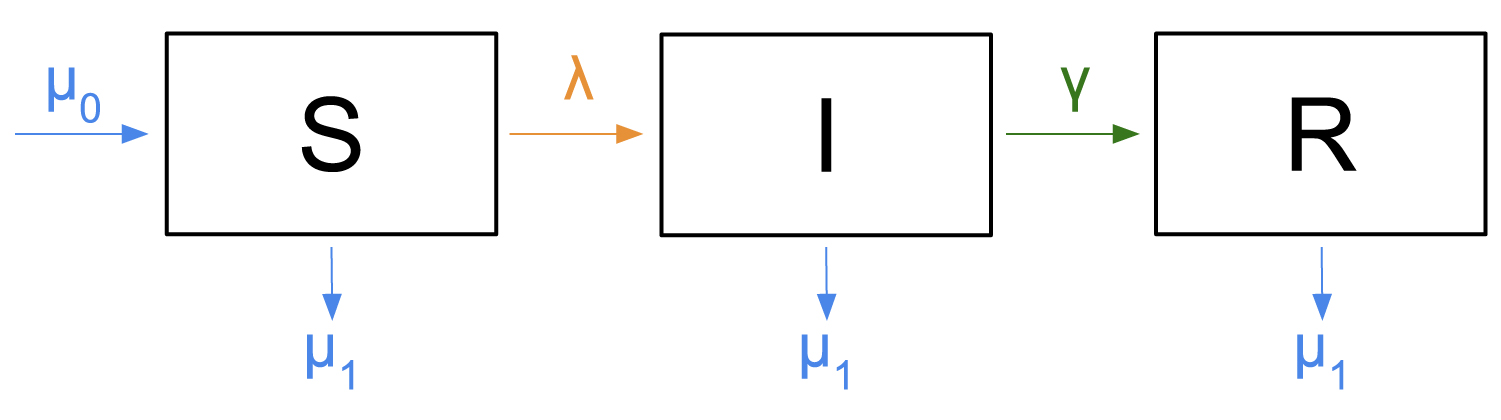
\includegraphics[width=\textwidth]{figures/SIR.jpg}\\
%		
%		\begin{eqnarray*}
%		\left\{
%		\begin{array}{lcl}
%			\dv{S}{t}  & = &  -\beta S + \lambda I \\
%			\tmspace{1mu}&& \\
%			\dv{I}{t} & = & \beta S - (\lambda + \gamma)I \\
%			\tmspace{1mu}&& \\
%			\dv{R}{t} & = & \gamma I
%		\end{array}
%		\right.
%		\end{eqnarray*}
%	\end{column}
%	\end{columns}
%}
%
%
%%\sframe{SIR model dynamics}{
%%	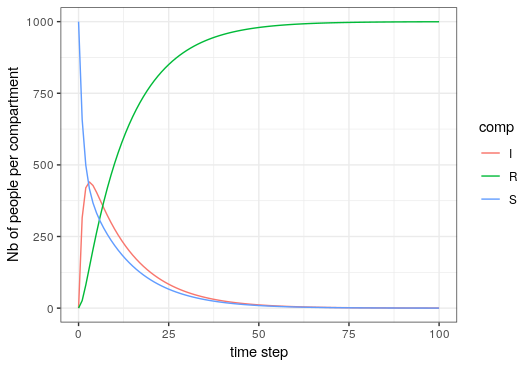
\includegraphics[width=\textwidth]{figures/SIR_dynamics.png}
%%}
%
%
%\sframe{ODE vs ABM}{
%	\begin{table}
% 	\begin{tabular}{ll}
% 		\thead{\head{ODE}} & \thead{\head{ABM}} \\
%		Equation-based & Individual-based \\
%		Generic mechanisms & Precise mechanisms \\
%		Population scale & Individual scale \\
%		Needs less resources & Computationally  expensive
%  	\end{tabular}
%  	\end{table}
%}
%
%
%\section{A Zombie situation}
%
%\sframe{An ODE model for our Zombie problem}{
%	\head{How could we model the Zombie invasion?}
%	
%	\begin{itemize}
%		\item Which mechanisms?
%		\item Which parameters?
%	\end{itemize}
%	
%	\bigskip
%	
%	\visible<2>{
%	\head{How can we assess our model's ability to reproduce the real data?}
%	
%	\begin{itemize}
%		\item Which metrics?
%		\item Which fitness function?
%	\end{itemize}
%	}
%}









\end{document}